% Preamble:
% \usepackage{tikz}
% \usepackage{xcolor}

\begin{figure}[ht]
\centering
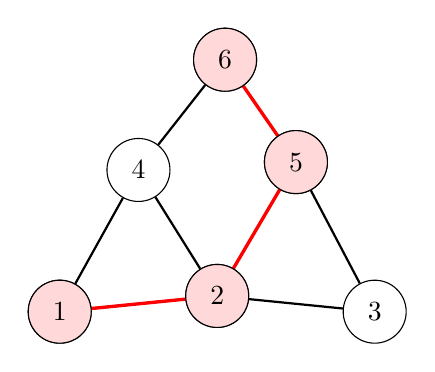
\begin{tikzpicture}[
  v/.style={circle, draw, minimum size=8mm},
  e/.style={thick},
  pathE/.style={very thick, red},
  pathV/.style={circle, draw, fill=red!15, minimum size=8mm}
]

% --- vertices ---
\node[v] (1) at (0,0)   {$1$};
\node[v] (2) at (2,0.2) {$2$};
\node[v] (3) at (4,0.0) {$3$};
\node[v] (4) at (1.0,1.8) {$4$};
\node[v] (5) at (3.0,1.9) {$5$};
\node[v] (6) at (2.1,3.2) {$6$};

% --- edges (graph) ---
\draw[e] (1)--(2);
\draw[e] (2)--(3);
\draw[e] (1)--(4);
\draw[e] (2)--(4);
\draw[e] (2)--(5);
\draw[e] (3)--(5);
\draw[e] (4)--(6);
\draw[e] (5)--(6);

% --- highlighted path: 1-2-5-6 ---
\draw[pathE] (1)--(2);
\draw[pathE] (2)--(5);
\draw[pathE] (5)--(6);

% highlight the path vertices (optional)
\node[pathV] at (1) {$1$};
\node[pathV] at (2) {$2$};
\node[pathV] at (5) {$5$};
\node[pathV] at (6) {$6$};

\end{tikzpicture}
\caption{A graph with the path $1 \to 2 \to 5 \to 6$ highlighted in red.}
\label{fig:path-highlight}
\end{figure}
